\documentclass[11pt,]{article}
\usepackage[left=1in,top=1in,right=1in,bottom=1in]{geometry}
\newcommand*{\authorfont}{\fontfamily{phv}\selectfont}
\usepackage[]{mathpazo}


  \usepackage[T1]{fontenc}
  \usepackage[utf8]{inputenc}



\usepackage{abstract}
\renewcommand{\abstractname}{}    % clear the title
\renewcommand{\absnamepos}{empty} % originally center

\renewenvironment{abstract}
 {{%
    \setlength{\leftmargin}{0mm}
    \setlength{\rightmargin}{\leftmargin}%
  }%
  \relax}
 {\endlist}

\makeatletter
\def\@maketitle{%
  \newpage
%  \null
%  \vskip 2em%
%  \begin{center}%
  \let \footnote \thanks
    {\fontsize{18}{20}\selectfont\raggedright  \setlength{\parindent}{0pt} \@title \par}%
}
%\fi
\makeatother




\setcounter{secnumdepth}{3}

\usepackage{longtable,booktabs}

\usepackage{graphicx,grffile}
\makeatletter
\def\maxwidth{\ifdim\Gin@nat@width>\linewidth\linewidth\else\Gin@nat@width\fi}
\def\maxheight{\ifdim\Gin@nat@height>\textheight\textheight\else\Gin@nat@height\fi}
\makeatother
% Scale images if necessary, so that they will not overflow the page
% margins by default, and it is still possible to overwrite the defaults
% using explicit options in \includegraphics[width, height, ...]{}
\setkeys{Gin}{width=\maxwidth,height=\maxheight,keepaspectratio}

\title{Técnicas de Ecología numérica aplicadas a la comunidad de
Chrysobalanaceae representada en la parcela permanente de Barro Colorado
Island (BCI)\\[2\baselineskip]  }



\author{\Large Melany Karina Ogando Matos\vspace{0.05in} \newline\normalsize\emph{Estudiante, Universidad Autónoma de Santo Domingo (UASD)}  }


\date{}

\usepackage{titlesec}

\titleformat*{\section}{\normalsize\bfseries}
\titleformat*{\subsection}{\normalsize\itshape}
\titleformat*{\subsubsection}{\normalsize\itshape}
\titleformat*{\paragraph}{\normalsize\itshape}
\titleformat*{\subparagraph}{\normalsize\itshape}

\titlespacing{\section}
{0pt}{36pt}{0pt}
\titlespacing{\subsection}
{0pt}{36pt}{0pt}
\titlespacing{\subsubsection}
{0pt}{36pt}{0pt}





\newtheorem{hypothesis}{Hypothesis}
\usepackage{setspace}

\makeatletter
\@ifpackageloaded{hyperref}{}{%
\ifxetex
  \PassOptionsToPackage{hyphens}{url}\usepackage[setpagesize=false, % page size defined by xetex
              unicode=false, % unicode breaks when used with xetex
              xetex]{hyperref}
\else
  \PassOptionsToPackage{hyphens}{url}\usepackage[unicode=true]{hyperref}
\fi
}

\@ifpackageloaded{color}{
    \PassOptionsToPackage{usenames,dvipsnames}{color}
}{%
    \usepackage[usenames,dvipsnames]{color}
}
\makeatother
\hypersetup{breaklinks=true,
            bookmarks=true,
            pdfauthor={Melany Karina Ogando Matos (Estudiante, Universidad Autónoma de Santo Domingo (UASD))},
             pdfkeywords = {ecología numérica, BCI, Chrysobalanaceae, correlación, agrupamiento,
biodiversidad},  
            pdftitle={Técnicas de Ecología numérica aplicadas a la comunidad de
Chrysobalanaceae representada en la parcela permanente de Barro Colorado
Island (BCI)\\[2\baselineskip]},
            colorlinks=true,
            citecolor=blue,
            urlcolor=blue,
            linkcolor=magenta,
            pdfborder={0 0 0}}
\urlstyle{same}  % don't use monospace font for urls

% set default figure placement to htbp
\makeatletter
\def\fps@figure{htbp}
\makeatother

\usepackage{pdflscape} \newcommand{\blandscape}{\begin{landscape}}
\newcommand{\elandscape}{\end{landscape}} \usepackage{float}
\floatplacement{figure}{H}
\newcommand{\beginsupplement}{ \setcounter{table}{0} \renewcommand{\thetable}{S\arabic{table}} \setcounter{figure}{0} \renewcommand{\thefigure}{S\arabic{figure}} }


% add tightlist ----------
\providecommand{\tightlist}{%
\setlength{\itemsep}{0pt}\setlength{\parskip}{0pt}}

\begin{document}
	
% \pagenumbering{arabic}% resets `page` counter to 1 
%
% \maketitle

{% \usefont{T1}{pnc}{m}{n}
\setlength{\parindent}{0pt}
\thispagestyle{plain}
{\fontsize{18}{20}\selectfont\raggedright 
\maketitle  % title \par  

}

{
   \vskip 13.5pt\relax \normalsize\fontsize{11}{12} 
\textbf{\authorfont Melany Karina Ogando Matos} \hskip 15pt \emph{\small Estudiante, Universidad Autónoma de Santo Domingo (UASD)}   

}

}








\begin{abstract}

    \hbox{\vrule height .2pt width 39.14pc}

    \vskip 8.5pt % \small 

\noindent Los patrones de dispersión y agrupamiento de las especies revelan
información acerca de como estas interactúan con el medio ambiente. El
objetivo de esta investigación es conocer el patrón de distribución de
las especies de Chrysobalanaceae que se encuentran representadas en BCI
utilizando técnicas de ecología númerica. Los métodos realizados
incluyen análisis de agrupamiento, técnicas de ordenación, medidas de la
diversidad y análisis de ecología espacial. Los resultados demostraron
que existe una correlación espacial inducida por las variables
ambientales. \emph{Licania }hypoleuca demostró ser una especie
indicadora para uno de los grupos formado por el análisis de
agrupamiento. Como se trata de datos censales se demostró la completitud
de la muestra por medio de estimadores de riqueza. Los sitios de BCI se
encuentran altamente correlacionados en función de las variables
ambientales, por lo que la riqueza por sitio es lo que caracteriza cada
uno de estos.


\vskip 8.5pt \noindent \emph{Keywords}: ecología numérica, BCI, Chrysobalanaceae, correlación, agrupamiento,
biodiversidad \par

    \hbox{\vrule height .2pt width 39.14pc}



\end{abstract}


\vskip 6.5pt


\noindent  \section{Introducción}\label{introducciuxf3n}

Conocer la dispersion y las formas de agrupamiento de los individuos de
una especie, es necesario para su conservacion (Condit et al., 1996,
Hubbell \& Foster (1992)). Las especies no son las mismas en todos los
lugares, y estos patrones de variación, en cada uno de los niveles de
diversidad: genes, especies y ecosistemas, es el objeto de estudio de la
biogeografía. Su objetivo es caracterizar la distribucion de las
especies en la actualidad y la variacion geografica de la diversidad en
términos de la interacción de los organismos con su ambiente (Lomolino,
Riddle, Whittaker, \& Brown, 2010). La similiridad es una medida simple
de la similitud de especies y sus abundancias. Es convencional decir que
es lo mismo alta diversidad con alta homogeneidad, lo que es equivalente
a poca dominancia (Magurran, 2004).

Los patrones de biodiversidad son el resultado de la combinacion de los
procesos internos de la comunidad de plantas y las condiciones externas
del ambiente (Sang \& Bai, 2008). Por ejemplo, la cantidad de nitrogeno
en el suelo puede ser asumida como una limitante directa en la
distribucion de las especies de plantas (Lange, Nobel, Osmond, \&
Ziegler, 2013). Numerosas especies de la familia Chrysobalanaceae poseen
preferencia por suelos húmedos (Regional Conservation (2020), Future
(2021), C. Sothers, Prance, Buerki, De Kok, \& Chase (2014), Grandtner
\& Chevrette (2013)).Esta es una familia de plantas de distribucion
pantropical, y cuenta con 18 géneros con 531 especies que se encuentra
un 80\% en el neotrópico.(G. Prance, 2014, Bardon et al. (2013)).

Las especies de Chrysobalaneceae son utilizadas de maneras distintas
para el tratamiento y como medicina de algunas enfermedades como la
malaria, epilepsia, diarrea y diabetes (Feitosa, Xavier, \& Randau,
2012). Sus usos son frecuentes en la región africana y surámericana,
donde son más abundantes (Feitosa et al., 2012). Posee diferentes usos
como: El aceite de sus frutos para pinturas y varnices, tambien su
madera como material de construccion, combustible y carbón. Ademas es
utilizada mezclada con arcilla para hacer vasijas de barro (G. Prance,
2014).

La parcela permanente de la isla de Barro Colorado es una reserva de
investigacion biologica a cargo del Smithsonian Tropical Research
Institute (Croat, 1978).\\
Segun Condit (1998) la distribucion de \emph{Hirtella americana} en la
parcela permanente de BCI se encuentra de manera irregular en pequeñas
areas isoladas. Sin embargo, los estudios realizados no han demostrado
que esta irregularidad se deba a variables ambientales. Croat (1978)
menciona que \emph{Hirtella americana} es una de las especies mayor
representadas por su densidad en este bosque.

Con el motivo de aplicar estudios de ecología numérica y aprender a
utilizarlos en futuras investigaciones, además de descubrir si existen
patrones de correlación entre la familia de plantas Chrysobalanaceae y
algunas variables ambientales, esta investigación tiene como objetivos
conocer la distribución espacial de las especies de la familia
Chrysobalanaceae, conoces si se agrupan en grupos discontinuos en
función de su composición, y reconocer si estos patrones se encuentran
relacionados con alguna variable ambiental. Además de identificar, en
caso de que existan, las tendencias de ordenación de la especies de
Chrysobalanaceae representadas en BCI y su correspondencia con las
variables del ambiente. Este estudio busca estimar la riqueza de la
familia Chrysobalanceae en la parcela permanente de Barro Colorado
Island y descubir la relación entre la diversidad alpha y las variables
ambientales, además de la relación de las especies con la diversidad
beta. Tambien identificar si los modelos de distribución de especies
predicen la ocurrencia de las especies representadas en el estudio.

Para realizar un estudio a fondo de la correlación entre esta familia y
las variables ambientales era necesario realizar multiples analisis de
ecología numerica, por esta razon se realizaron analisis de
agrupamiento, tecnicas de ordenacion, analaisis de diversidad y ecología
espacial. Ya que cada uno responde a distintas preguntas de
investigación. Este estudio intenta resumir los patrones de diversidad
asociados a la familia Chrysobalanaceae en la parcela permanente de BCI.

\section{Metodología}\label{metodologuxeda}

\subsection{Obtención de los datos}\label{obtenciuxf3n-de-los-datos}

Los datos fueron obtenidos del censo realizado durante el 2010 por el
Smithsonian Tropical Research Institute en la parcela permanente de
Barro Colorado Island en el lago Gatún, Panamá (S. Hubbell, Condit, \&
Foster, 2010). En este censo, se contabilizaron todas las árboles con
troncos de al menos 10mm de Diámetro de Altura de Pecho, y estos fueron
identificados y marcados. Esta parcela cuenta con 50 hectáreas dividida
en 50 cuadros de 1 hectárea cada una.

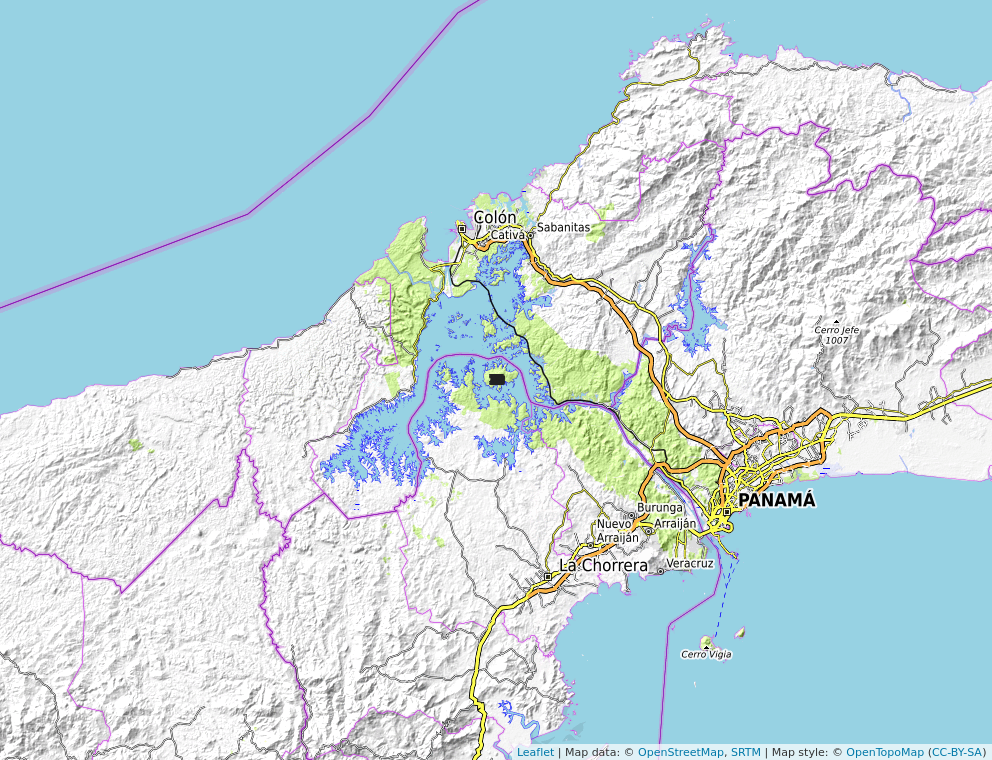
\includegraphics{mapa_cuadros_panama.png}\{width = 80\%\}

Los datos utilizados en esta investigación fueron administrados a través
del repositorio Batlle (2020). Estos datos continenen la matriz de
comunidad y la matriz ambiental. En la matriz de comunidad se extrajeron
los datos de la familia Chrysobalanaceae.

\subsection{Análisis estadístico}\label{anuxe1lisis-estaduxedstico}

Para conocer los patrones de agrupamiento según la composición de
especies de Chrysobalanaceae se realizó un análisis de agrupamiento
tomando en consideración cuatro técnicas jerarquicas y aglomerativas
(Borcard, Gillet, Legendre, \& others, 2011, Krebs (2014)), las cuales
fueron: por enlace simple,por enlace completo, por enlace promedio
(UPGMA) y por el método de Ward. Los datos de la matriz de comunidad
fueron normalizados y se calculó la distancia euclídea, para luego
proceder a realizar las técnicas de agrupamiento.

Para conocer el patrón de organización de la familia Chrysobalanaceae y
seleccionar el dendrograma que mejor explica las relaciones entre las
especies de esta familia, se realizaron pruebas de distancia cofenética;
y para conocer el número de grupos óptimo se calculó la anchura de
siluetas. Por medio de Bootstrap multiescalar se revisaron los datos
obtenidos en los métodos anteriores. Para evaluar la relación de los
grupos obtenidos con las variables ambientales se utilizó una prueba de
igualdad de promedios por t student y la prueba no paramétrica de la
suma de rangos de Wilcoxon (medianas). Además, se realizó un análisis de
especies indicadoras mediante la prueba de IndVal y un analisis de
especies con preferencia por hábitat mediante el coeficiente de
correlación biserial puntual (Phi).

Las técnicas de ordenación consisten en colocar objetos o variables en
un espacio donde cada uno representa una dimensión (Borcard et al.,
2011). Los gráficos generados mediante estos análisis muestran una
relación ordenada de las variables formando un diagrama de dispersión
(Legendre \& Legendre, 2012, Legendre \& Gallagher (2001)).

A fin de detectar las tendencias de ordenación de las especies de la
familia Chrysobalanaceae se utilizaron diferentes técnicas de tipo
restringida y no restringida. El análisis de componentes principales
(PCA) se realizó para variables ambientales utilizando solo las
variables numéricas y escalándolas a puntuaciones Z para generar una
matriz de correlaciones; para las variables de la matriz de comunidad
los datos fueron transformados basados en Hellinger. El análisis de
correspondencia (CA) se realizó calculando las distancias de los objetos
en CHI cuadradro. La técnicas de ordenación restringida utilizada fue un
análisis de correspondencia canónica (CCA).

Para el análisis de la diversidad Alpha se calcularon los números de
diversidad Alpha y los ratios de Hill como se encuentra explicado por
Krebs (2014) y Borcard et al. (2011). Los sitios que poseían solo una
especie fueron excluidos. Posteriormente, se realizó un análisis de
correlacion de pearson con las variables ambientales seleccionadas, para
conocer si existe asociación con la diversidad Alpha. Con el objetivo de
medir la diversidad de especies de una localidad cuando solo se tienen
una muestra de la riqueza total de la comunidad, se utilizó el enfoque
asintótico no paramétrico de Chao. La diversidad beta calculada con los
datos de presencia/ausencia de las especies nos dice cúantas más
especies están presentes en toda el área que en un sitio individual
(Borcard et al., 2011). La contribución local de los sitios y las
especies a la diversidad beta fue realizada siguiendo los procedimientos
indicados por Borcard et al. (2011).

Uno de los fundamentos de la ecología espacial es comprender como el
espacio impacta en la estructura de la comunidad (Cantrell, Cosner, \&
Ruan, 2010). La autocorrelación espacial es una medida de la similaridad
o disimilaridad de dos sitios cercanos con relación a los pares
seleccionados aleatoriamente {[}borcard2011numerical{]}. El análisis de
correlacción espacial se realizó siguiendo la metodología descrita por
Batlle (2020). En primer lugar, los datos de la matriz de comunidad
fueron transformados midiendo la distancia Hellinger, y se generó la
vecindad para la matriz ambiental. Entonces, la autocorrelación de las
especies y las variables ambientales se midió a partir de un
correlograma. Posteriormente, se eliminaron las tendencias espaciales de
autocorrelación transformando la matriz de comunidad Hellinger en una
matriz de posiciones XY, para luego realizar una prueba Mantel de
correlograma. De igual forma, se evaluó la autocorrelación espacial por
I de Moran sin tomar en cuenta las tendencias espaciales.

Los análisis fueron realizados en la consola de RStudio (R Core Team,
2020) administrada por José Ramón Martínez Batlle. Para acceder a la
consola se realizó mediante el navegador Google Chrome en una
computadora personal de prestaciones básicas. Los paquetes utilizados
para los diferentes análisis fueron Oksanen et al. (2019), R. Kindt \&
Coe (2005), Wickham (2017) y De Caceres \& Legendre (2009).

\section{Resultados}\label{resultados}

La familia Chrysobalanaceae se encuentra representada en BCI por un
total de 4,821 individuos formada por las especies \emph{Hirtella
americana}, \emph{Hirtella triandra}, \emph{Licania platypus} y
\emph{Licania hypoleuca} (/ref\{tab:tabla\_abun\}. La especie más
abundante fue \emph{Hirtella triandra}, que representa un 90\% de la
composición de la familia en BCI.

{[}Tabla de abundancias de las especies de Chrysobalanaceae en
BCI\label{tab:tabla_abun}{]}

\begin{longtable}[]{@{}ll@{}}
\toprule
Especie & Abundancia\tabularnewline
\midrule
\endhead
\emph{Hirtella triandra} & 4408\tabularnewline
\emph{Licania platypus} & 251\tabularnewline
\emph{Licania hypoleuca} & 141\tabularnewline
\emph{Hirtella americana} & 21\tabularnewline
\bottomrule
\end{longtable}

Los análisis de agrupamiento por medio de las cuatro técnicas mostraron
grupos similares, con un grupo consistente en todas las técnicas formado
por los sitios 24, 25, 29 y 30. Los dendrogramas que mostraron mayor
correlación cofenética fueron los creados por los métodos de enlace
completo y enlace promedio (UPGMA). El número de grupos obtenido
mediante el cálculo de anchura de silueta fue de dos para los
dendrogramas generados por enlace completo, por enlace pormedio (UPGMA)
y por Ward.

El mapa de calor generado para los dendrogramas muestra ligeramente la
apariencia de tres grupos, sin embargo el análisis mediante boostrap
multiescalar refuerza la partición en solo dos grupos para UPGMA, Ward y
por enlace completo. Ya que los dendrogramas generados por UPGMA y por
enlace completo mostraron resultados muy similares, los dendrogramas
utilizados para posteriores análisis fueron los generados por medio de
agrupamiento por enlace completo y Ward para dos grupos óptimos
\ref{clusters}. El grupo uno formado por 46 sitios y el grupo dos
formado por 4 sitios \ref{mapagrupos}.

\begin{figure}
\centering
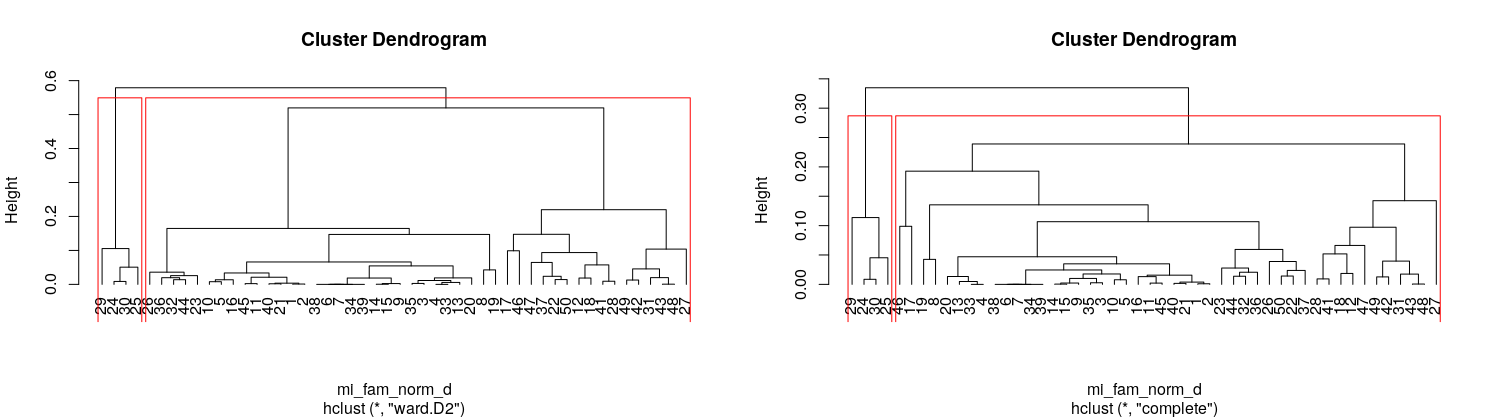
\includegraphics[width=1.00000\textwidth]{Clusters.png}
\caption{Dendrogramas generados por análisis de
agrupamiento\label{clusters}}
\end{figure}

\begin{figure}
\centering
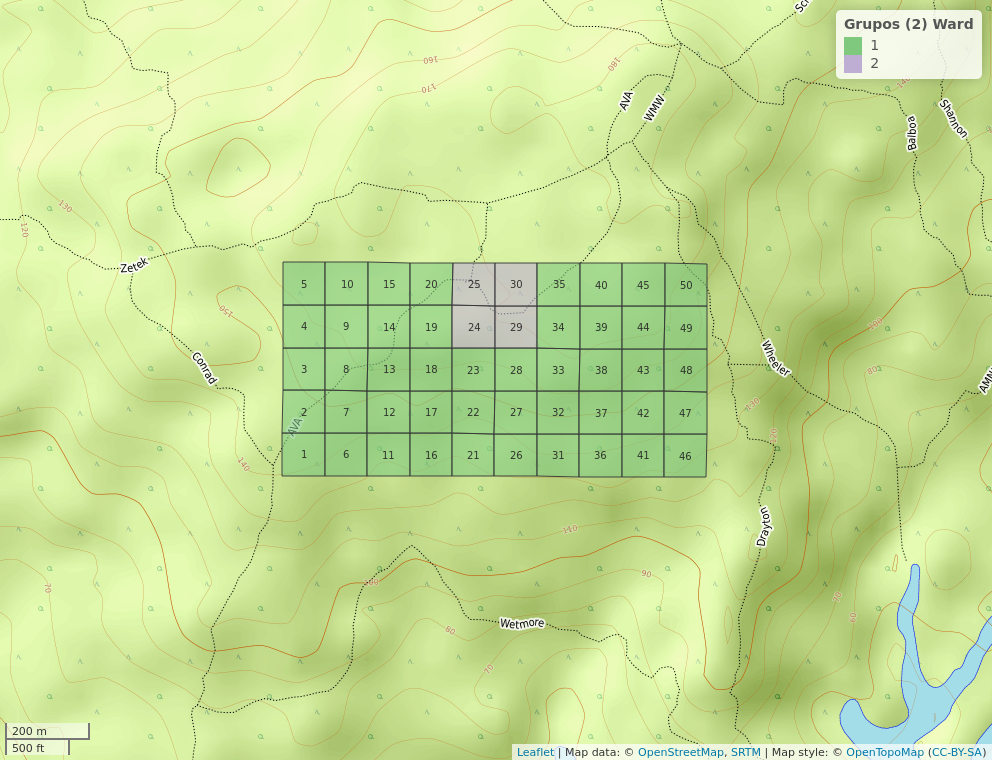
\includegraphics[width=0.80000\textwidth]{mapa_ward_k2.png}
\caption{Mapa según grupos generados por análisis de
agrupamiento\label{mapagrupos}}
\end{figure}

Las pruebas de igualdad de promedios realizadas por medio de t-student y
la suma de rangos de Wilcoxon mostró que las variables heterogeneidad
ambiental, Nitrógeno y elevación media muestran relación significativa
con los grupos formados por medio del análisis de agrupamiento.

Los análisis de especies indicadoras o con preferencia por determinados
hábitats dio como resultado que \emph{Licania hypoleuca} parece ser una
especie indicadora para el grupo 2 (formado por los sitios 24, 25, 29 y
30).

Mediante el cálculo de los factores de inflación (VIF) de las variables
de suelo y ambientales se escogió un grupo reducido de variables que
tuvieran poca correlación entre ellas con un VIF menor de 10. Las
variables escogidos fueron Aluminio, Cobre, Manganeso, Nitrógeno, pH,
Nitrógeno mineralizado, elevación media, heterogeneidad ambiental y
orientación media.

El análisis de componentes principales para los datos de variables
ambientales seleccionadas dio como resultado que los sitios se asocian
en dos grupos distintivos, sin embargo estos grupos no se corresponden
con los generados por medio del análisis de agrupamiento por enlace
completo (\ref{pcagruop}).

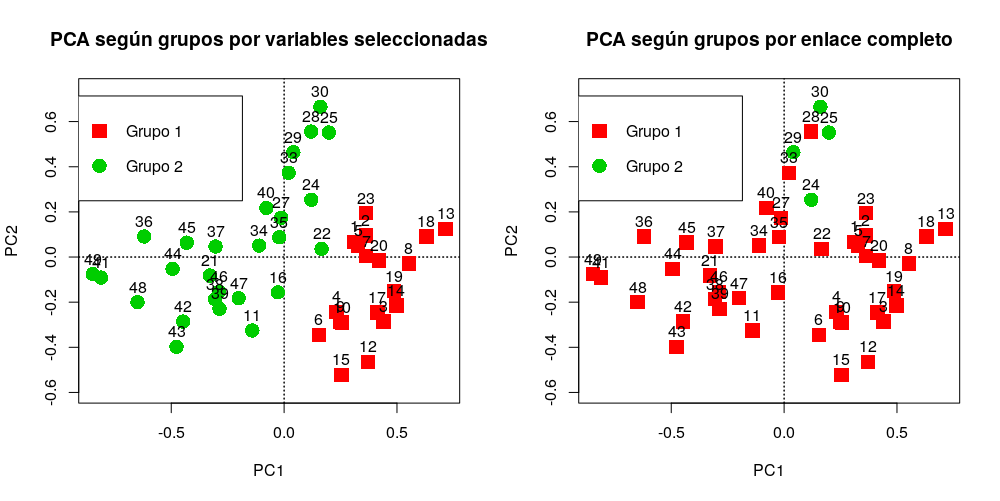
\includegraphics{PCA_porgrupos.png}\{widtht = 80\%\}

El análisis de componentes principales (PCA) aplicado a la matriz de
comunidad muestra la relación de \emph{Licania hypoleuca} con los sitios
del grupo 2 del análisis de agrupamiento generado por enlace completo
\ref{pcaespecies}, al igual que en el análisis de correspondecia. Esta
especie parece asociarse de manera inversa con la abundancia de
Manganeso. Las especies \emph{Hirtella triandra} e \emph{Hirtella
americana} presentan correlación inversa, pues los vectores se muestran
en direcciones completamente opuestas.

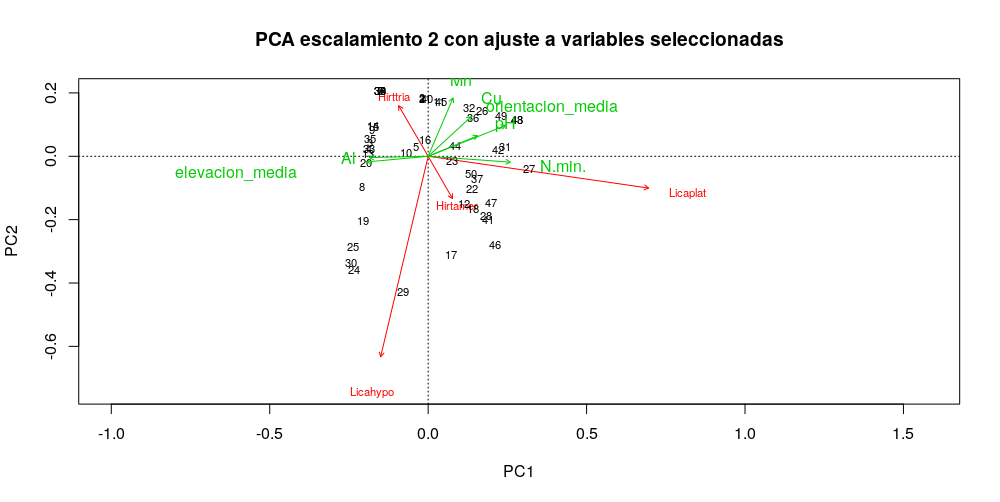
\includegraphics{PCA_especies.png}\{widtht = 80\%\}

Los resultados del análisis de correspondencia canónica explican un 47\%
de los datos y en la grafica se puede verificar que \emph{Hirtella
triandra} es la especie con mayor abundancia, pues se encuentra en el
centro del gráfico. También se muestra que \emph{Licania platypus} se
encuentra muy correlacionada con la abundancia de nitrógeno mineralizado
(\ref{triplotrda}).

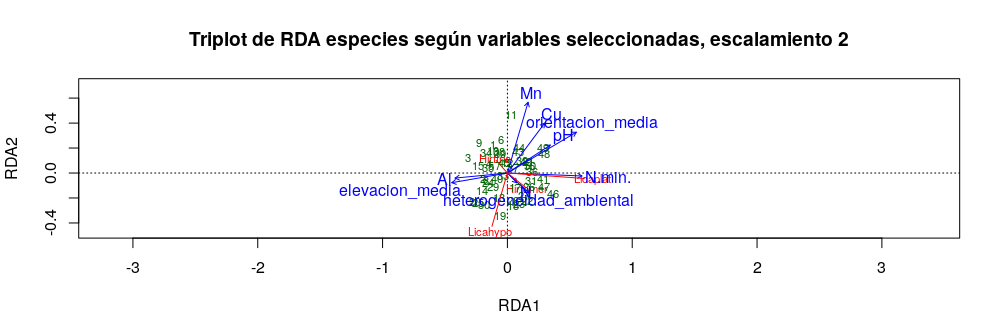
\includegraphics{triplotRDA.png}\{widtht = 80\%\}

Las variables ambientales Magnesio, Zinc, Nitrógeno mineralizado y
geomorfología de interfluvio mostraron relación con los números de Hill.
Mientras que pH y Nitrógeno parecen estar correlacionadas con la equidad
de Pielou (\ref{diversidadalpha}). El trabajo de muestreo realizado en
BCI con relación a la familia Chrysobalanaceae se estima que representa
un 100\% de completitud de la muestra, según los estimadores de Chao
\ref{extrapolacion}, por lo que podemos afirmar que esta familia se
encuentra muy bien representada en BCI.

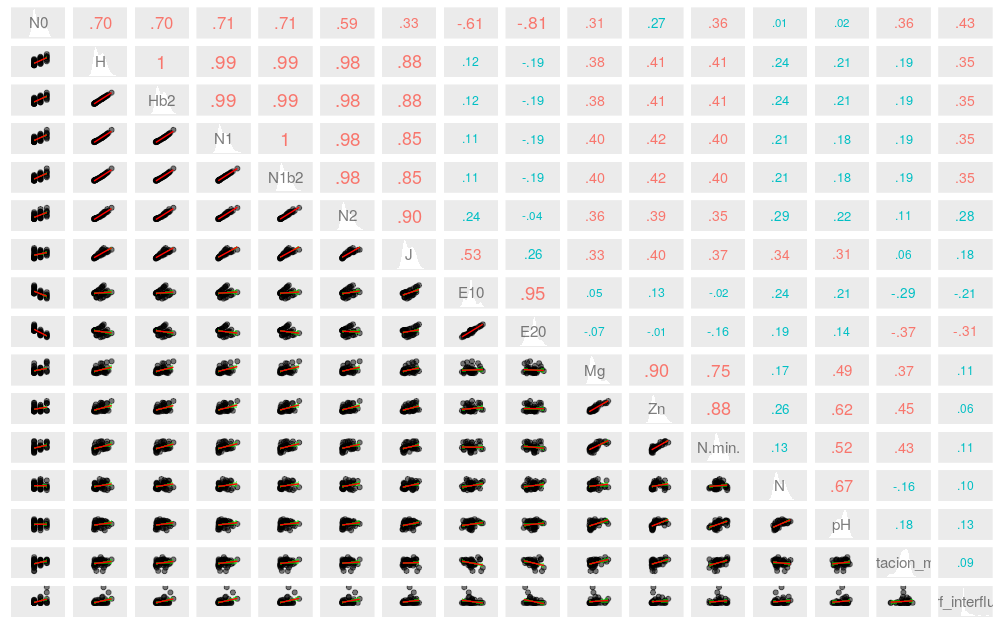
\includegraphics{diversidadalpha.png}\{widtht = 80\%\}

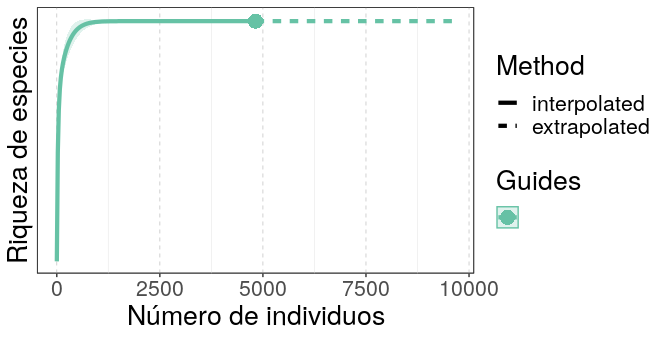
\includegraphics{Extrapolacion_mifamilia.png}\{widtht = 80\%\}

Sin embargo, al realizar la estimación de la riqueza por medio de los
estimadores de Chao para los grupos generados en el análisis de
agrupamiento, se estima que el grupo 1 se encuentra representado en un
100\%, pero para el grupo 2 es necesario aumentar el esfuerzo de
muestreo. Esto puede deberse a la desigualdad del número de sitios en
los grupos.

La diversidad beta multiplicativa disminuye mientras aumenta la
importancia de la abundancia más que la riqueza, esto se debe a la
autocorrelación espacial de los sitios, y demuestra que la diversidad de
la comunidad está marcada por la presencia de especies indicadoras. Las
especies que muestran contribución a la diversidad beta son
\emph{Licania hypoleuca} y \emph{Licania platypus}, mientras que ninguno
de los sitios resultó como contribuyente.

Mediante la prueba de correlograma las variables Boro, Calcio, Magnesio,
Zinc, Nitrógeno, pH y Nitrógeno mineralizado mostraron correlación en
múltiples órdenes (\ref{correlograma}). La prueba Mantel sin tendencias
de autocorrelación muestra que en los residuos la correlación no es
significativa, por lo que parece que hay una dependencia espacial
inducida por las variables ambientales. El I de moran aplicado a la
matriz sin tendencia espacial dio como resultado que \emph{Licania
hypoleuca} e \emph{Hirtella triandra} se encuentran en un patrón
aglomerativo (\textbackslash{}ref\{lisamaps). Las variable que muestra
un patrón aglomerativo común es la elevación media.

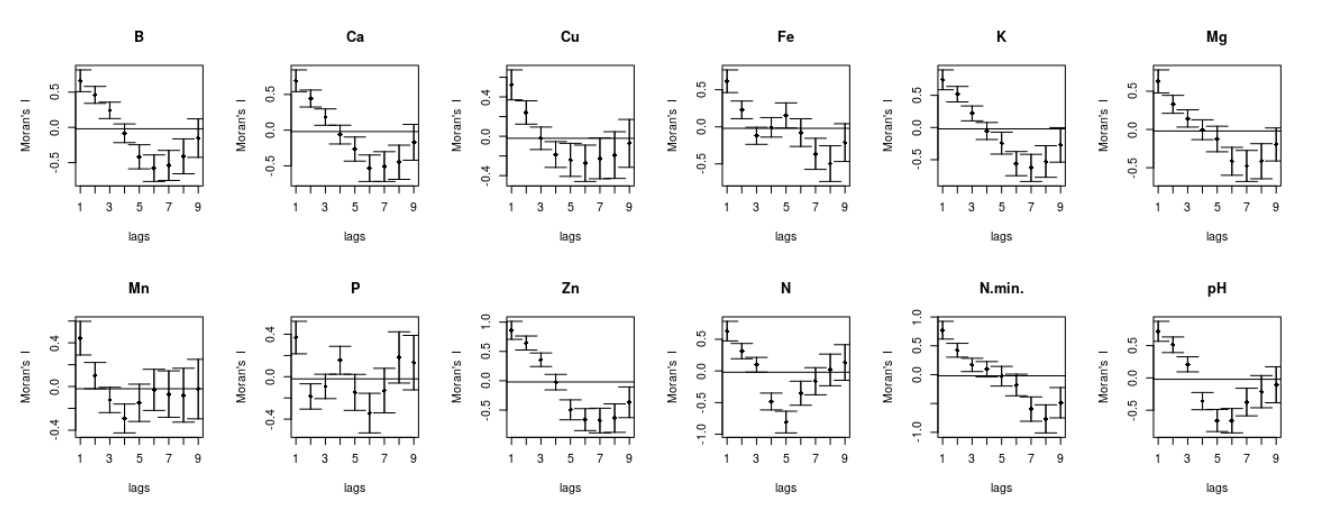
\includegraphics{correlogramavariables.png}\{widtht = 80\%\}

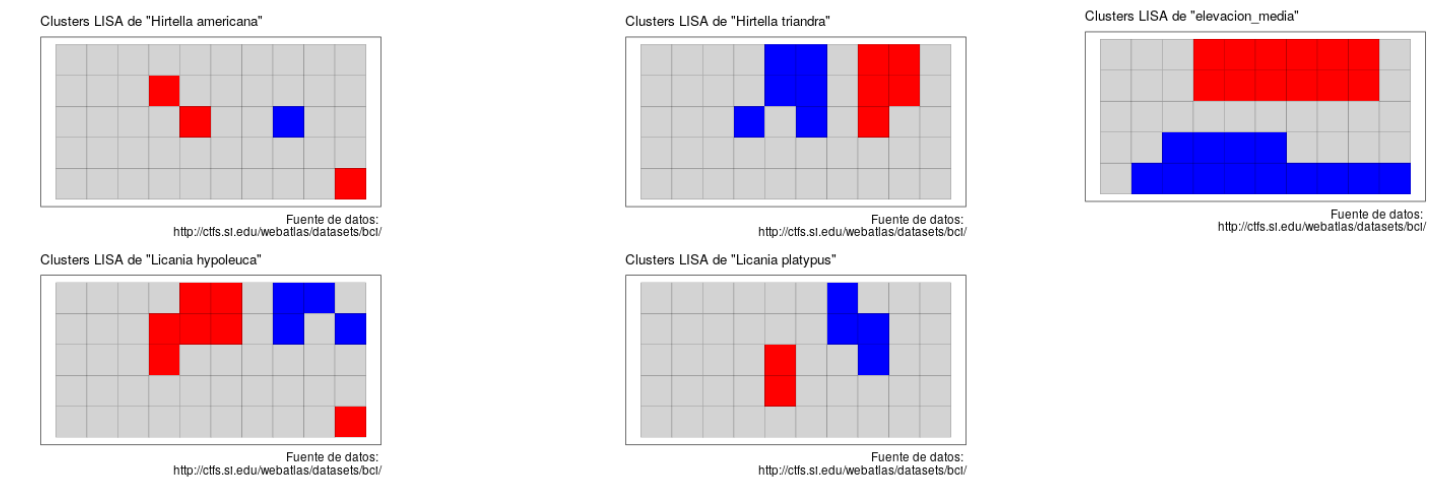
\includegraphics{clusterlisaespecies.png}\{widtht = 80\%\}

\section{Discusión}\label{discusiuxf3n}

La composición de especies de la familia Chrysobalanaceae en BCI no
parece organizarse en patrones discontinuos, aunque los análisis de
agrupamiento muestran un grupo formado por los sitios 24, 25, 29 y 30
que se caracteriza por la abundancia de \emph{Licania hypoleuca}.

Las técnicas de análisis de ordenación al comparar sitios y especies
demuestra, al igual que el análisis de agrupamiento, que los sitios del
grupo 2 se encuentran correlacionados con la abundancia de \emph{Licania
hypoleuca}. Esta tendencia de ordenación parece asociarse de manera
inversa con la abundancia de Manganeso, además este análisis muestra que
la abundancia de \emph{Licania platypus} se correlaciona con el
nitrógeno mineralizado.

Debido a que el método de muestreo utilizado para generar la base de
datos usada en esta investigación se trata de un censo, es por esto que
el análisis de estimación de riqueza muestra una alta completitud de la
muestra. Las especies raras son el mayor contribuyente a la diversidad
beta de la comunidad.

Los datos parecen mostrar una correlación espacial inducida alta. Sin
embargo, al general los mapas Lisa las especies \emph{Licania hypoleuca}
e \emph{Hirtella triandra} solo parecen mostrar un patrón aglomerado con
respecto a la orientación media.

Se recomienda aplicar otras técnicas de ecología numérica a estos datos
para comparar los resultados de la variables selecionadas, y verificar
los modelos de agrupamiento obtenidos además de como se relacionan con
las variables ambientales.

\section{Agradecimientos}\label{agradecimientos}

Agradezco al profesor José Martínez Batlle por sus enseñanzas y su apoyo
en el análisis de esta investigación. También al Smithsonian Tropical
Research Institute por la obtención y el suministro de los datos.

\section{Información de soporte}\label{informaciuxf3n-de-soporte}

\section{\texorpdfstring{\emph{Script}
reproducible}{Script reproducible}}\label{script-reproducible}

\section*{Referencias}\label{referencias}
\addcontentsline{toc}{section}{Referencias}

\hypertarget{refs}{}
\hypertarget{ref-bardon2013origin}{}
Bardon, L., Chamagne, J., Dexter, K. G., Sothers, C. A., Prance, G. T.,
\& Chave, J. (2013). Origin and evolution of chrysobalanaceae: Insights
into the evolution of plants in the neotropics. \emph{Botanical Journal
of the Linnean Society}, \emph{171}(1), 19--37.

\hypertarget{ref-jose_ramon_martinez_batlle_2020_4402362}{}
Batlle, J. R. M. (2020). biogeografia-master/scripts-de-analisis-BCI:
Long coding sessions (Version v0.0.0.9000).
\url{https://doi.org/10.5281/zenodo.4402362}

\hypertarget{ref-borcard2011numerical}{}
Borcard, D., Gillet, F., Legendre, P., \& others. (2011).
\emph{Numerical ecology with r} (Vol. 2). Springer.

\hypertarget{ref-cantrell2010spatial}{}
Cantrell, R. S., Cosner, C., \& Ruan, S. (2010). \emph{Spatial ecology}.
CRC Press.

\hypertarget{ref-condit1998tropical}{}
Condit, R. (1998). \emph{Tropical forest census plots: Methods and
results from barro colorado island, panama and a comparison with other
plots}. Springer Science \& Business Media.

\hypertarget{ref-condit1996species}{}
Condit, R., Hubbell, S. P., Lafrankie, J. V., Sukumar, R., Manokaran,
N., Foster, R. B., \& Ashton, P. S. (1996). Species-area and
species-individual relationships for tropical trees: A comparison of
three 50-ha plots. \emph{Journal of Ecology}, 549--562.

\hypertarget{ref-croat1978flora}{}
Croat, T. B. (1978). \emph{Flora of barro colorado island}. Stanford
University Press.

\hypertarget{ref-indicspeciesR}{}
De Caceres, M., \& Legendre, P. (2009). Associations between species and
groups of sites: Indices and statistical inference. In \emph{Ecology}.
Retrieved from \url{http://sites.google.com/site/miqueldecaceres/}

\hypertarget{ref-feitosa2012chrysobalanaceae}{}
Feitosa, E. A., Xavier, H. S., \& Randau, K. P. (2012).
Chrysobalanaceae: Traditional uses, phytochemistry and pharmacology.
\emph{Revista Brasileira de Farmacognosia}, \emph{22}(5), 1181--1186.

\hypertarget{ref-PfafLrigida}{}
Future, P. for a. (2021). Licania rigida (benth). Retrieved November 11,
2021, from
\url{https://pfaf.org/user/Plant.aspx?LatinName=Licania+rigida}

\hypertarget{ref-grandtner2013dictionary}{}
Grandtner, M. M., \& Chevrette, J. (2013). \emph{Dictionary of trees,
volume 2: South america: Nomenclature, taxonomy and ecology}. Academic
Press.

\hypertarget{ref-hubbell1992short}{}
Hubbell, S. P., \& Foster, R. B. (1992). Short-term dynamics of a
neotropical forest: Why ecological research matters to tropical
conservation and management. \emph{Oikos}, 48--61.

\hypertarget{ref-Hubbell2010Forest}{}
Hubbell, S., Condit, R., \& Foster, R. (2010). Forest census plot on
barro colorado island. Retrieved November 30),, from
\url{http://ctfs.si.edu/webatlas/datasets/bci/}

\hypertarget{ref-biodiversityR}{}
Kindt, R., \& Coe, R. (2005). \emph{Tree diversity analysis. a manual
and software for common statistical methods for ecological and
biodiversity studies}. Retrieved from
\url{http://www.worldagroforestry.org/output/tree-diversity-analysis}

\hypertarget{ref-krebs1999ecological}{}
Krebs, C. J. (2014). \emph{Ecological methodology} (3rd ed.).

\hypertarget{ref-lange2013physiological}{}
Lange, O. L., Nobel, P. S., Osmond, C. B., \& Ziegler, H. (2013).
\emph{Physiological plant ecology iii: Responses to the chemical and
biological environment} (Vol. 12). Springer Science \& Business Media.

\hypertarget{ref-legendre2001ecologically}{}
Legendre, P., \& Gallagher, E. D. (2001). Ecologically meaningful
transformations for ordination of species data. \emph{Oecologia},
\emph{129}(2), 271--280.

\hypertarget{ref-legendre2012numerical}{}
Legendre, P., \& Legendre, L. (2012). \emph{Numerical ecology}.
Elsevier.

\hypertarget{ref-lomolino2017biogeography}{}
Lomolino, M. V., Riddle, B. R., Whittaker, R. J., \& Brown, J. H.
(2010). \emph{Biogeography}.

\hypertarget{ref-magurran2004measuring}{}
Magurran, A. (2004). Measuring biological diversity. 2004. \emph{Malden:
Blackwell}.

\hypertarget{ref-veganR}{}
Oksanen, J., Blanchet, F. G., Friendly, M., Kindt, R., Legendre, P.,
McGlinn, D., \ldots{} Wagner, H. (2019). \emph{Vegan: Community ecology
package}. Retrieved from \url{https://CRAN.R-project.org/package=vegan}

\hypertarget{ref-prance2014chrysobalanaceae}{}
Prance, G. (2014). Chrysobalanaceae. In \emph{Flowering plants.
eudicots} (pp. 19--28). Springer.

\hypertarget{ref-RStudio}{}
R Core Team. (2020). \emph{R: A language and environment for statistical
computing}. Retrieved from \url{https://www.R-project.org/}

\hypertarget{ref-ircCicaco}{}
Regional Conservation, T. I. for. (2020). Chrysobalanus icaco,
chrysobalanaceae. Retrieved November 11, 2021, from
\url{https://regionalconservation.org/beta/nfyn/plantdetail.asp?tx=Chryicac\&tx=Chryicac}

\hypertarget{ref-sang2008vascular}{}
Sang, W., \& Bai, F. (2008). Vascular diversity patterns of forest
ecosystem before and after a 43-year interval under changing climate
conditions in the changbaishan nature reserve, northeastern china. In
\emph{Forest ecology} (pp. 115--130). Springer.

\hypertarget{ref-sothers2014taxonomic}{}
Sothers, C., Prance, G. T., Buerki, S., De Kok, R., \& Chase, M. W.
(2014). Taxonomic novelties in neotropical chrysobalanaceae: Towards a
monophyletic couepia. \emph{Phytotaxa}, \emph{172}(2), 176--200.

\hypertarget{ref-tidyverseR}{}
Wickham, H. (2017). \emph{Tidyverse: Easily install and load the
'tidyverse'}. Retrieved from
\url{https://CRAN.R-project.org/package=tidyverse}




\newpage
\singlespacing 
\end{document}
